%! TeX program = lualatex
\documentclass[a4paper]{article} 

% packages
\usepackage{microtype}      % Slightly tweak font spacing for aesthetics
\usepackage[english]{babel} % Language hyphenation and typographical rules
\usepackage[final, colorlinks = true, urlcolor = black, linkcolor = black, citecolor = black]{hyperref} 
\usepackage{changepage}     % adjust margins on the fly
\usepackage{multicol}

\usepackage[backend=biber, style=numeric, date=iso, urldate=iso]{biblatex}
\addbibresource{references.bib}
\DeclareFieldFormat{urldate}{Accessed on: #1}

\usepackage{fontspec}
\setmainfont{EB Garamond}
\setmonofont[Scale=MatchLowercase]{Deja Vu Sans Mono}

\usepackage{minted}
\usemintedstyle{algol_nu}
\usepackage{xcolor}

\usepackage{pgfplots}
\pgfplotsset{width=\textwidth,compat=1.9}

\usepackage{caption}
\newenvironment{code}{\captionsetup{type=listing}}{}
\captionsetup[listing]{skip=0pt}
\setlength{\abovecaptionskip}{5pt}
\setlength{\belowcaptionskip}{5pt}

\usepackage[yyyymmdd]{datetime}
\renewcommand{\dateseparator}{--}

\usepackage{tikz}
\usetikzlibrary{trees}

\usepackage{titlesec}
% \titleformat{\section}{\LARGE\bfseries}{}{}{}[\titlerule]
% \titleformat{\subsection}{\Large\bfseries}{}{0em}{}
% \titlespacing{\subsection}{0em}{-0.7em}{0em}
%
% \titleformat{\subsubsection}{\large\bfseries}{}{0em}{$\bullet$ }
% \titlespacing{\subsubsection}{1em}{-0.7em}{0em}

% margins
\addtolength{\hoffset}{-2.25cm}
\addtolength{\textwidth}{4.5cm}
\addtolength{\voffset}{-3.25cm}
\addtolength{\textheight}{5cm}
\setlength{\parskip}{0pt}
\setlength{\parindent}{0in}
% \setcounter{secnumdepth}{0}

\begin{document}
\hrule \medskip
\begin{minipage}{0.295\textwidth} 
    \vfill
    \raggedright
    \footnotesize 
    \begin{tabular}{@{}l l} % Define a two-column table with left alignment
        Name: & Andrew Hayes \\
        Student ID: & 21321503 \\
        Programme: & 4BCT \\
    \end{tabular}
    \vfill
\end{minipage}
\begin{minipage}{0.4\textwidth} 
    \centering 
    \Large 
    \vfill
    \textbf{CT4101}
    \vfill
\end{minipage}
\begin{minipage}{0.295\textwidth} 
    \raggedleft
    \vfill
    \today
    \vfill
\end{minipage}
\smallskip
\hrule 
\begin{center}
    \normalsize
    Assignment 01: Classification Using Scikit-Learn
\end{center}
\hrule

\section{Description of Algorithms}
\subsection{Algorithm 1: Random Forest}
% Detailed description of algorithm 1.
% Clearly describe each of your chosen scikit-learn algorithm implementations in turn, paying special attention to discussing the two hyperparameters that you have chosen to tune for each algorithm.
% You should write a maximum of 1 page per algorithm. 

\textbf{Random decision forest} is a supervised machine learning algorithm that can be used for both classification \& regression that builds upon the \textbf{decision tree} algorithm by combining several decision trees to generate labels for a dataset.
An implementation of this algorithm for classification is provided in scikit-learn as \mintinline{python}{sklearn.ensemble.RandomForestClassifier} \supercite{scikit_randomforestclassifier}.
While it can be used for regression as well as classification, I will only be referring to its use as a classification algorithm in this assignment, as regression is not relevant to the wildfire classification task at hand.
\\\\
Since the random decision forest algorithm builds upon the decision tree algorithm, it is first necessary to explain briefly what decision trees are and how they work.
A decision tree can be thought of a series of internal nodes (i.e., nodes which are not leaf nodes) that contain a question which separates the input data.
The decision tree is traversed from root to leaf for each instance being classified, where the leaf node to which we arrive is the label for that instance.
For example, a decision tree might be used to determine whether or not a living thing is a mammal, where each internal node is a question that helps to separate non-mammalian data instances from mammalian, and each leaf node is a label stating whether or not the living thing is a mammal.
Each internal node should narrow down the final label as much as possible i.e., each question should give us the maximum information about the instance and should be arranged in the order that narrows it down as quickly as possible.

\begin{figure}[H]
    \centering
    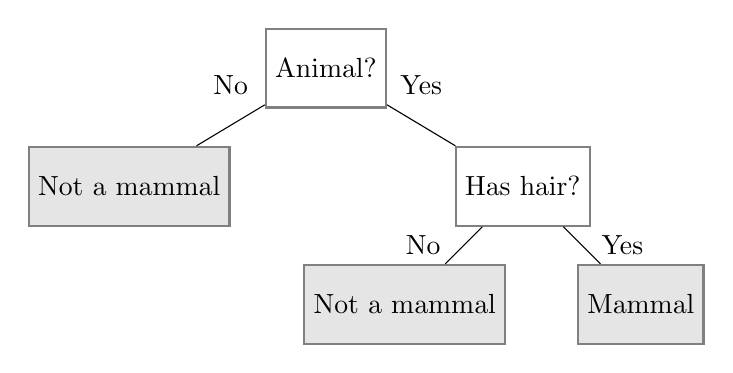
\begin{tikzpicture}[
        every node/.style={rectangle, draw=black!50, thick, minimum size=1cm},
        level 1/.style={sibling distance=5cm},
        level 2/.style={sibling distance=3cm}
    ]

    % Internal Nodes
    \node[fill=white] {Animal?}
        child { node[fill=gray!20] {Not a mammal}  edge from parent node[above, draw=none] {No} }
        child { node[fill=white] {Has hair?}
            child { node[fill=gray!20] {Not a mammal} edge from parent node[left, draw=none] {No} }
            child { node[fill=gray!20] {Mammal} edge from parent node[right, draw=none] {Yes} }
            edge from parent node[above, draw=none] {Yes}
        };

    \end{tikzpicture}
    \caption{Simplified Decision Tree to Determine Whether a Creature is a Mammal}
\end{figure}

Decision trees have many advantages: they are visualisable by humans and aren't ``black-box'', they can model non-linear relationships easily, and they are robust to outliers.
However, they have their disadvantages, including instability (small changes in the training data can significantly alter the tree structure) and in particular \textbf{overfitting}: when the algorithm fits too exactly to the training data, making it incapable of generalising to unseen data.
An extreme example of overfitting would be if the example decision tree above started to ask far too specific questions, e.g. ``Is it a dolphin'', ``Is it a human''. 
While this would have excellent performance \& accuracy on the test data, it would not work at all for an animal it hadn't encountered before.
\\\\
Random forests work by combining many decision trees into a forest, thus improving accuracy \& reducing overfitting by averaging multiple trees, reducing variance and leading to better generation.
These decision trees are each generated using random, potentially overlapping subsets of the data training data.
While the original random forest algorithm worked by taking the most popular label decided on by the set of trees \supercite{breiman}, the scikit-learn \mintinline{python}{RandomForestClassifier} works by taking a probability estimate for each label from each tree and averaging these to find the best label\supercite{scikit_ensembles}.

\begin{figure}[H]
    \centering
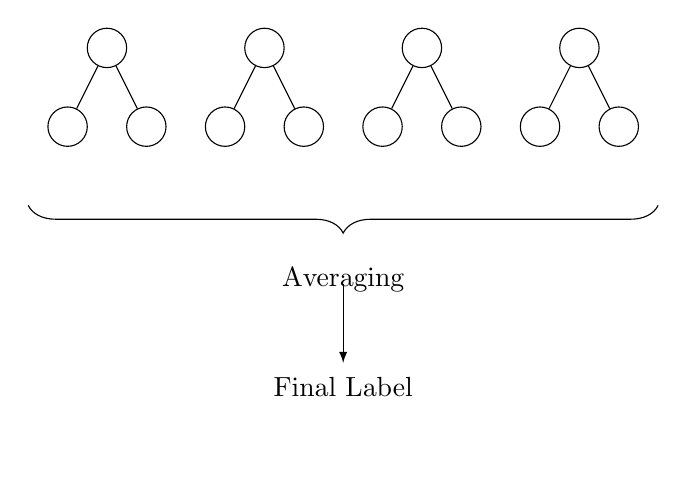
\begin{tikzpicture}[every node/.style={circle, draw, minimum size=0.5cm}]

    % Binary Trees
    \node (tree1) at (0,0) {};
    \node (tree1l) at (-0.5,-1) {};
    \node (tree1r) at (0.5,-1) {};
    \draw (tree1) -- (tree1l) {};
    \draw (tree1) -- (tree1r) {};
    
    \node (tree2) at (2,0) {};
    \node (tree2l) at (1.5,-1) {};
    \node (tree2r) at (2.5,-1) {};
    \draw (tree2) -- (tree2l) {};
    \draw (tree2) -- (tree2r) {};

    \node (tree3) at (4,0) {};
    \node (tree3l) at (3.5,-1) {};
    \node (tree3r) at (4.5,-1) {};
    \draw (tree3) -- (tree3l) {};
    \draw (tree3) -- (tree3r) {};
    
    \node (tree4) at (6,0) {};
    \node (tree4l) at (5.5,-1) {};
    \node (tree4r) at (6.5,-1) {};
    \draw (tree4) -- (tree4l) {};
    \draw (tree4) -- (tree4r) {};

    % Averaging Bracket
    \draw[decorate,decoration={brace,amplitude=10pt,mirror}] (-1,-2) -- (7,-2) node[below, midway, draw=none] {Averaging};

    % Final Label
    % \node at (4,-3) {final label};
    % \draw[->] (4,-2) -- (4,-2.5);
    \draw[-latex] (3,-3) -- (3,-4); % Adjust the coordinates as needed
    \node[draw=none] at (3,-4.3) {Final Label};
\end{tikzpicture}
\caption{Random Forest Algorithm Example Diagram (with scikit-learn Averaging)}
\end{figure}

I chose the random forest classifier because it is resistant to overfitting, works well with complex \& non-linear data like the wildfire data in question, and offers a wide variety of hyperparameters for tuning.
\\\\
\colorbox{yellow}{TODO:} add hyperparameter details for tuning
% https://scikit-learn.org/stable/modules/ensemble.html#forest

% \subsubsection{Why I Chose This Algorithm}
%
% \subsubsection{Hyperparameter Details for Tuning}
% \subsubsection{Hyperparameter 1: Name}
% \subsubsection{Hyperparameter 2: Name}


\subsection{Algorithm 2: C-Support Vector Classification}

% \subsection{Algorithm 2: Gaussian Na\"ive Bayes}
% I chose this algorithm as I thought it could give an interesting contrast to my other chosen algorithm as Na\"ive Bayes is, generally speaking, not a very good choice for this kind of classification problem with environmental data.
% This is because Na\"ive Bayes assumes \textit{feature independence}, which is certainly not true with the wildfire data provided for this assignment: for example, the features \verb|temp| \& \verb|humidity| are naturally going to be correlated, as are the features \verb|rainfall| \& \verb|drought_code|.

% Detailed description of algorithm 1.
% Clearly describe each of your chosen scikit-learn algorithm implementations in turn, paying special attention to discussing the two hyperparameters that you have chosen to tune for each algorithm.
% You should write a maximum of 1 page per algorithm. 
%
% \subsubsection{Why I Chose This Algorithm}
%
% \subsubsection{Hyperparameter Details for Tuning}
% \subsubsection{Hyperparameter 1: Name}
% \subsubsection{Hyperparameter 2: Name}
%
% \section{Model Training \& Evaluation}
%
% \section{Conclusion}
%
% \bibliographystyle{plain}
% \bibliography{references}

\nocite{*}
\printbibliography
\end{document}
